\documentclass[tikz,border=0pt]{standalone}
\usepackage{fontspec}
\hyphenpenalty=10000
\exhyphenpenalty=10000
\setmainfont[Path=../fonts/,BoldFont=Poppins-SemiBold.ttf,ItalicFont=Poppins-Italic.ttf]{Poppins-Regular.ttf}
\usepackage{pgfplots}
\pgfplotsset{compat=1.18}
\usetikzlibrary{calc,arrows.meta}
\definecolor{ink}{HTML}{161b22}
\definecolor{text}{HTML}{353535}
\definecolor{muted}{HTML}{646c74}
\definecolor{line}{HTML}{d7dadd}
\definecolor{wash}{HTML}{f6f6f6}
\definecolor{tint}{HTML}{e6ecef}
\definecolor{link}{HTML}{1d63b7}
\definecolor{local}{HTML}{376c97}
\definecolor{api}{HTML}{995d46}
\definecolor{cloud}{HTML}{7b649b}
\definecolor{match}{HTML}{7d9fc4}
\definecolor{miss}{HTML}{e0e3e5}
\begin{document}
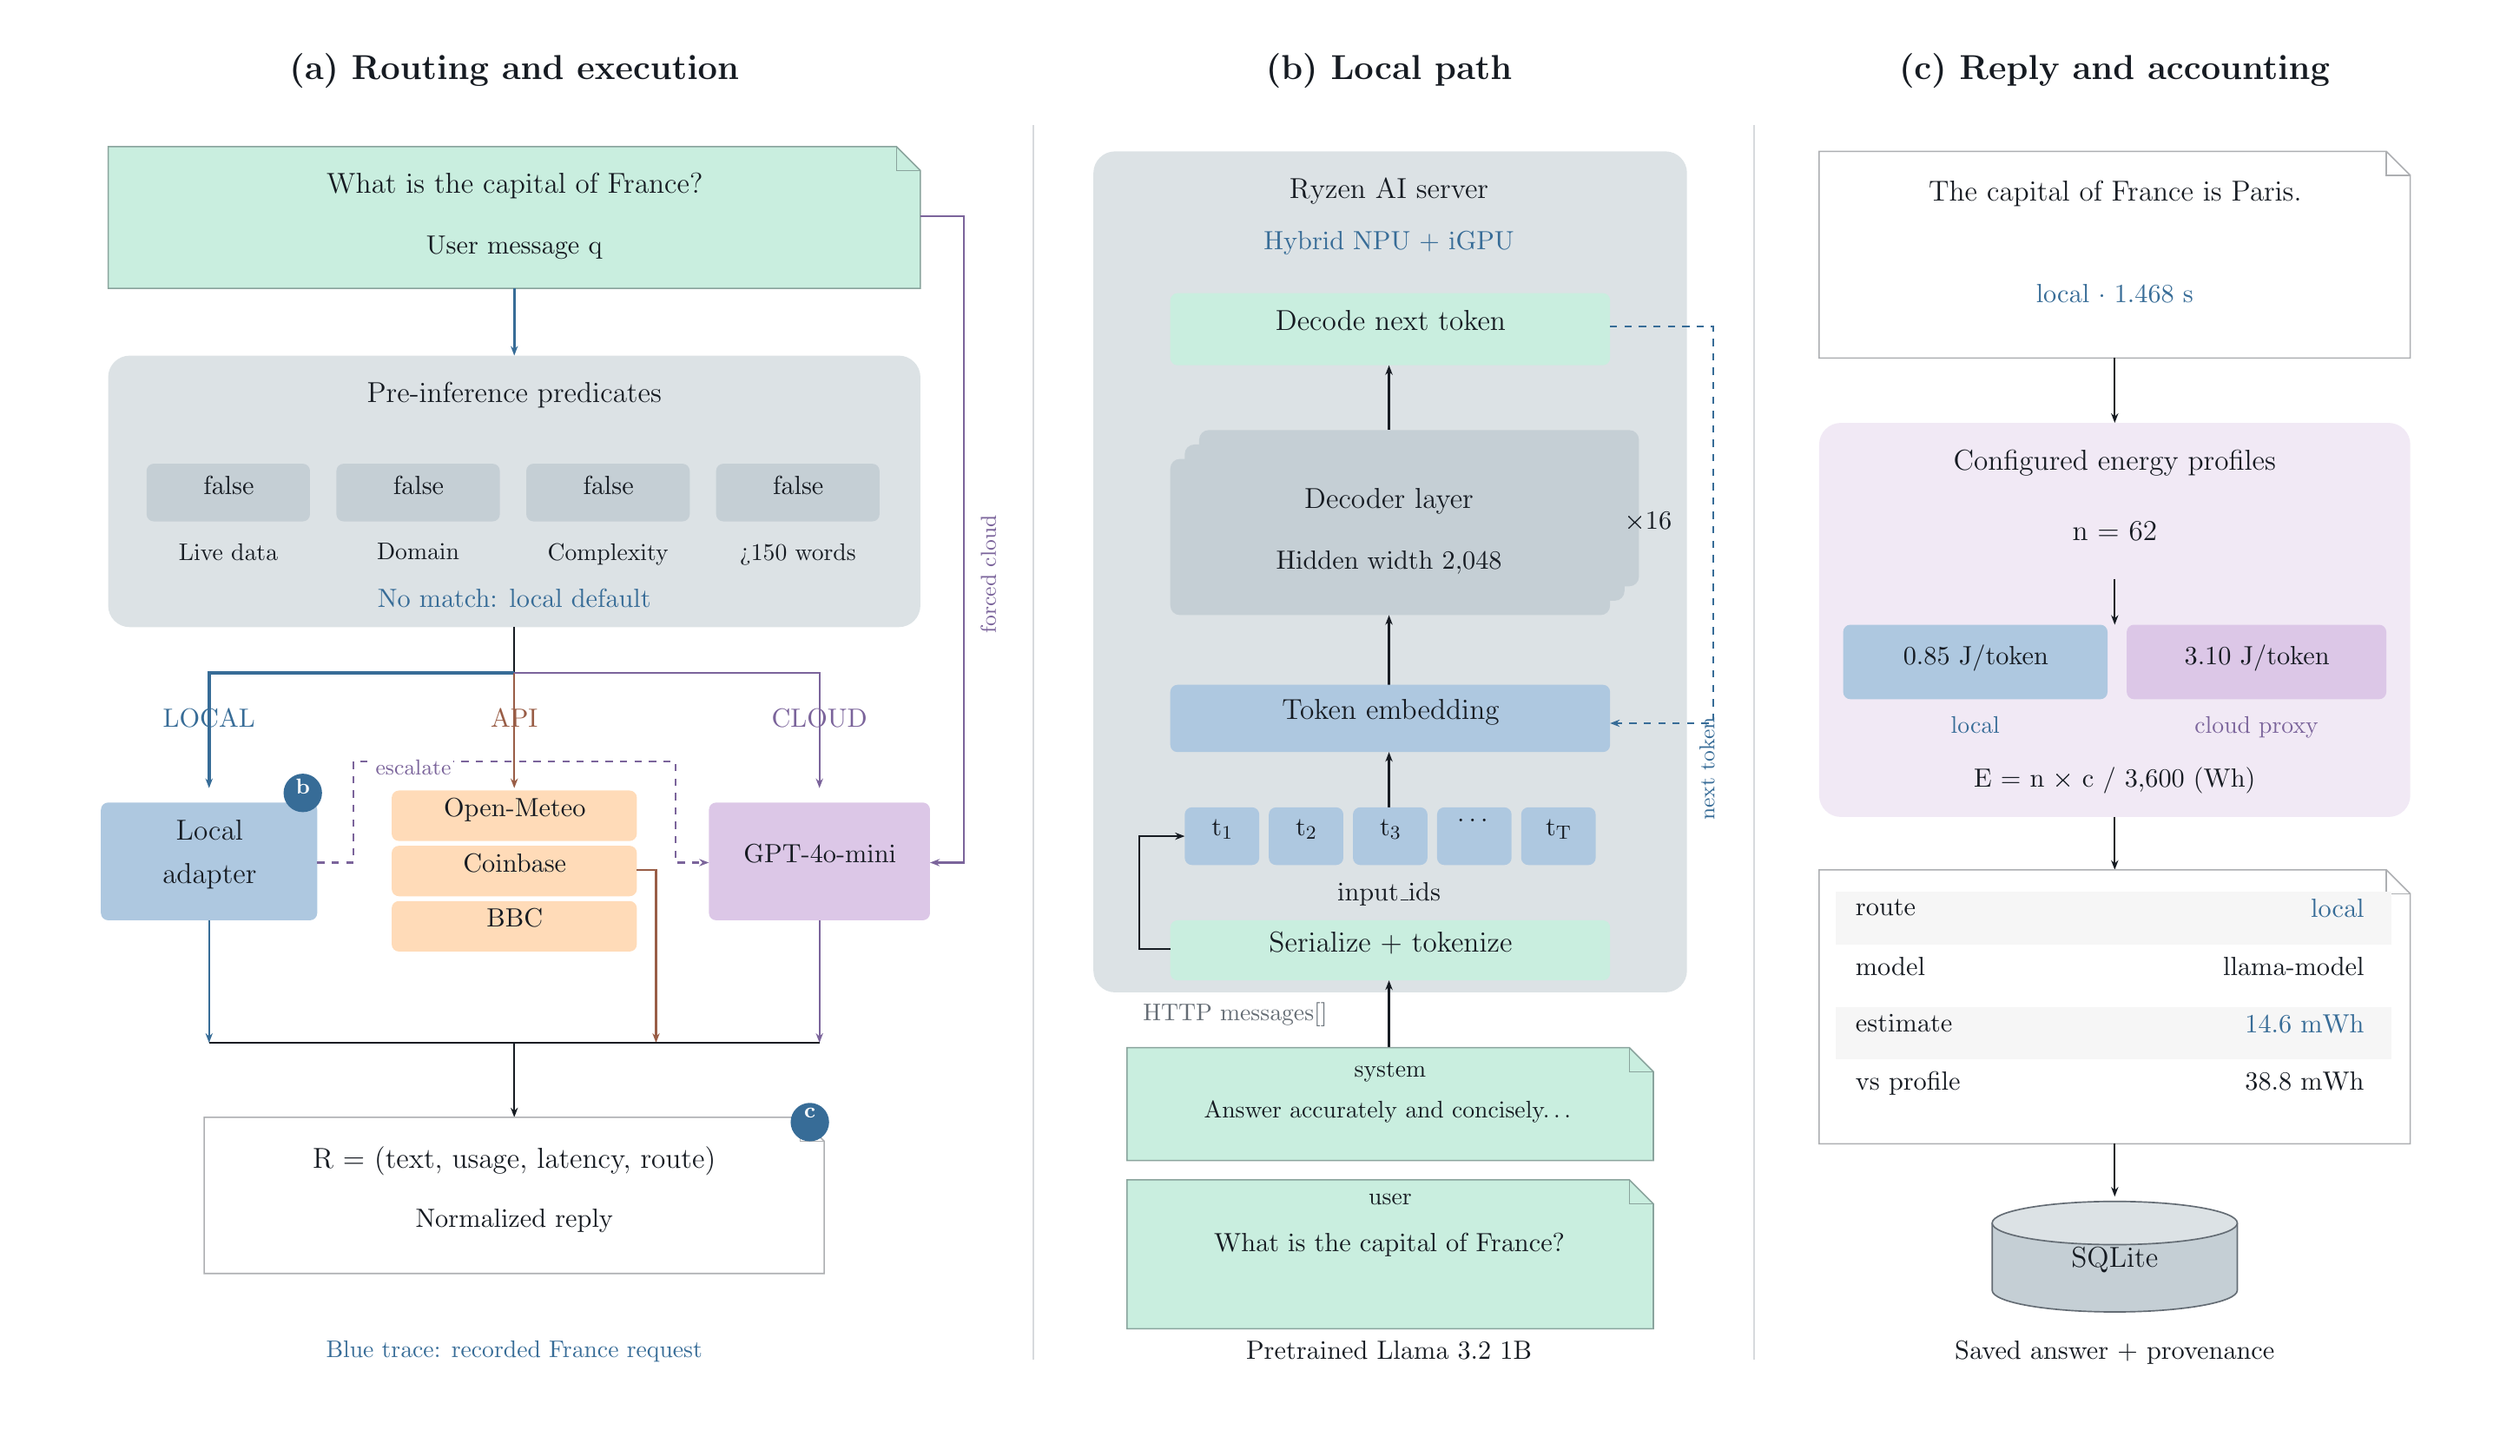
\begin{tikzpicture}[x=1pt,y=-1pt]
\path[use as bounding box] (0,0) rectangle (1020,575);
\definecolor{group}{HTML}{DCE2E5}
\definecolor{operation}{HTML}{C5CFD5}
\definecolor{mint}{HTML}{C9EEDF}
\definecolor{blueplane}{HTML}{AEC8E0}
\definecolor{pinkplane}{HTML}{F6D5DE}
\definecolor{peachplane}{HTML}{FFDBB8}
\definecolor{purpleplane}{HTML}{DCC7E7}
\node[anchor=north west,inner sep=0pt,text=ink,align=left,font=\fontsize{14}{21.0}\selectfont,anchor=north] at (204,12) {\textbf{(a) Routing and execution}};
\path[fill=mint,draw=mint!65!ink,line width=.55pt] (35,51) -- (363,51) -- (373,61) -- (373,110) -- (35,110) -- cycle;
\draw[mint!65!ink,line width=.45pt] (363,51) -- (363,61) -- (373,61);
\node[anchor=north west,inner sep=0pt,text=ink,align=center,font=\fontsize{13}{19.5}\selectfont,text width=310pt] at (49.0,62) {What is the capital of France?};
\node[anchor=north west,inner sep=0pt,text=ink,align=left,font=\fontsize{10.5}{15.75}\selectfont,anchor=north] at (204,88) {User message q};
\draw[-{Stealth[length=4pt,width=3pt]},line width=1.2pt,draw=local] (204,110) -- (204,138);
\path[fill=group,draw=none,line width=.6pt,rounded corners=9pt] (35,138) rectangle (373,251);
\node[anchor=north west,inner sep=0pt,text=ink,align=left,font=\fontsize{12.5}{18.75}\selectfont,anchor=north] at (204,149) {Pre-inference predicates};
\path[fill=operation,draw=none,line width=.6pt,rounded corners=3pt] (51,183) rectangle (119,207);
\node[anchor=north west,inner sep=0pt,text=ink,align=center,font=\fontsize{10.5}{15.75}\selectfont,text width=58pt] at (56.0,187.9125) {false};
\node[anchor=north west,inner sep=0pt,text=ink,align=left,font=\fontsize{9.7}{14.549999999999999}\selectfont,anchor=north] at (85,216) {Live data};
\path[fill=operation,draw=none,line width=.6pt,rounded corners=3pt] (130,183) rectangle (198,207);
\node[anchor=north west,inner sep=0pt,text=ink,align=center,font=\fontsize{10.5}{15.75}\selectfont,text width=58pt] at (135.0,187.9125) {false};
\node[anchor=north west,inner sep=0pt,text=ink,align=left,font=\fontsize{9.7}{14.549999999999999}\selectfont,anchor=north] at (164,216) {Domain};
\path[fill=operation,draw=none,line width=.6pt,rounded corners=3pt] (209,183) rectangle (277,207);
\node[anchor=north west,inner sep=0pt,text=ink,align=center,font=\fontsize{10.5}{15.75}\selectfont,text width=58pt] at (214.0,187.9125) {false};
\node[anchor=north west,inner sep=0pt,text=ink,align=left,font=\fontsize{9.7}{14.549999999999999}\selectfont,anchor=north] at (243,216) {Complexity};
\path[fill=operation,draw=none,line width=.6pt,rounded corners=3pt] (288,183) rectangle (356,207);
\node[anchor=north west,inner sep=0pt,text=ink,align=center,font=\fontsize{10.5}{15.75}\selectfont,text width=58pt] at (293.0,187.9125) {false};
\node[anchor=north west,inner sep=0pt,text=ink,align=left,font=\fontsize{9.7}{14.549999999999999}\selectfont,anchor=north] at (322,216) {>150 words};
\node[anchor=north west,inner sep=0pt,text=local,align=left,font=\fontsize{10.7}{16.049999999999997}\selectfont,anchor=north] at (204,235) {No match: local default};
\draw[line width=0.8pt,draw=ink] (204,251) -- (204,270);
\draw[-{Stealth[length=4pt,width=3pt]},line width=1.3pt,draw=local] (204,270) -- (77,270) -- (77,318);
\draw[-{Stealth[length=4pt,width=3pt]},line width=0.8pt,draw=api] (204,270) -- (204,318);
\draw[-{Stealth[length=4pt,width=3pt]},line width=0.8pt,draw=cloud] (204,270) -- (331,270) -- (331,318);
\node[anchor=north west,inner sep=0pt,text=local,align=left,font=\fontsize{10.5}{15.75}\selectfont,anchor=north] at (77,285) {LOCAL};
\node[anchor=north west,inner sep=0pt,text=api,align=left,font=\fontsize{10.5}{15.75}\selectfont,anchor=north] at (204,285) {API};
\node[anchor=north west,inner sep=0pt,text=cloud,align=left,font=\fontsize{10.5}{15.75}\selectfont,anchor=north] at (331,285) {CLOUD};
\path[fill=blueplane,draw=none,line width=.6pt,rounded corners=3pt] (32,324) rectangle (122,373);
\node[anchor=north west,inner sep=0pt,text=ink,align=center,font=\fontsize{12}{18.0}\selectfont,text width=80pt] at (37.0,331) {Local\\adapter};
\fill[local] (116,320) circle (8pt);
\node[anchor=north west,inner sep=0pt,text=white,align=left,font=\fontsize{9}{13.5}\selectfont,anchor=north] at (116,314) {\textbf{b}};
\path[fill=peachplane,draw=none,line width=.6pt,rounded corners=3pt] (153,319) rectangle (255,340);
\node[anchor=north west,inner sep=0pt,text=ink,align=center,font=\fontsize{10.8}{16.200000000000003}\selectfont,text width=92pt] at (158.0,322.21) {Open-Meteo};
\path[fill=peachplane,draw=none,line width=.6pt,rounded corners=3pt] (153,342) rectangle (255,363);
\node[anchor=north west,inner sep=0pt,text=ink,align=center,font=\fontsize{10.8}{16.200000000000003}\selectfont,text width=92pt] at (158.0,345.21) {Coinbase};
\path[fill=peachplane,draw=none,line width=.6pt,rounded corners=3pt] (153,365) rectangle (255,386);
\node[anchor=north west,inner sep=0pt,text=ink,align=center,font=\fontsize{10.8}{16.200000000000003}\selectfont,text width=92pt] at (158.0,368.21) {BBC};
\path[fill=purpleplane,draw=none,line width=.6pt,rounded corners=3pt] (285,324) rectangle (377,373);
\node[anchor=north west,inner sep=0pt,text=ink,align=center,font=\fontsize{10.8}{16.200000000000003}\selectfont,text width=82pt] at (290.0,341.21) {GPT-4o-mini};
\draw[-{Stealth[length=4pt,width=3pt]},line width=0.8pt,draw=cloud] (373,80) -- (391,80) -- (391,349) -- (377,349);
\node[anchor=north west,inner sep=0pt,text=cloud,align=left,font=\fontsize{9}{13.5}\selectfont,anchor=north,rotate=90] at (398,229) {forced cloud};
\draw[-{Stealth[length=4pt,width=3pt]},line width=0.8pt,draw=cloud,dashed] (122,349) -- (137,349) -- (137,307) -- (271,307) -- (271,349) -- (285,349);
\node[anchor=north west,inner sep=0pt,text=cloud,align=left,font=\fontsize{8.7}{13.049999999999999}\selectfont,anchor=north,fill=white,inner sep=1pt] at (162,305) {escalate};
\draw[-{Stealth[length=4pt,width=3pt]},line width=0.8pt,draw=local] (77,373) -- (77,424);
\draw[-{Stealth[length=4pt,width=3pt]},line width=0.8pt,draw=api] (255,352) -- (263,352) -- (263,424);
\draw[-{Stealth[length=4pt,width=3pt]},line width=0.8pt,draw=cloud] (331,373) -- (331,424);
\draw[line width=0.8pt,draw=ink] (77,424) -- (331,424);
\draw[-{Stealth[length=4pt,width=3pt]},line width=0.8pt,draw=ink] (204,424) -- (204,455);
\path[fill=white,draw=white!65!ink,line width=.55pt] (75,455) -- (323,455) -- (333,465) -- (333,520) -- (75,520) -- cycle;
\draw[white!65!ink,line width=.45pt] (323,455) -- (323,465) -- (333,465);
\node[anchor=north west,inner sep=0pt,text=ink,align=left,font=\fontsize{11.5}{17.25}\selectfont,anchor=north] at (204,467) {R = (text, usage, latency, route)};
\node[anchor=north west,inner sep=0pt,text=ink,align=left,font=\fontsize{11}{16.5}\selectfont,anchor=north] at (204,493) {Normalized reply};
\fill[local] (327,457) circle (8pt);
\node[anchor=north west,inner sep=0pt,text=white,align=left,font=\fontsize{9}{13.5}\selectfont,anchor=north] at (327,451) {\textbf{c}};
\node[anchor=north west,inner sep=0pt,text=local,align=left,font=\fontsize{10}{15.0}\selectfont,anchor=north] at (204,548) {Blue trace: recorded France request};
\draw[line,line width=.65pt] (420,42) -- (420,556);
\node[anchor=north west,inner sep=0pt,text=ink,align=left,font=\fontsize{14}{21.0}\selectfont,anchor=north] at (568,12) {\textbf{(b) Local path}};
\path[fill=group,draw=none,line width=.6pt,rounded corners=9pt] (445,53) rectangle (692,403);
\node[anchor=north west,inner sep=0pt,text=ink,align=left,font=\fontsize{12.5}{18.75}\selectfont,anchor=north] at (568,64) {Ryzen AI server};
\node[anchor=north west,inner sep=0pt,text=local,align=left,font=\fontsize{10.8}{16.200000000000003}\selectfont,anchor=north] at (568,86) {Hybrid NPU + iGPU};
\path[fill=mint,draw=none,line width=.6pt,rounded corners=3pt] (477,112) rectangle (660,142);
\node[anchor=north west,inner sep=0pt,text=ink,align=center,font=\fontsize{12}{18.0}\selectfont,text width=173pt] at (482.0,118.9) {Decode next token};
\draw[-{Stealth[length=4pt,width=3pt]},line width=0.8pt,draw=ink] (568,169) -- (568,142);
\path[fill=operation,draw=none,line width=.6pt,rounded corners=4pt] (489,169) rectangle (672,234);
\path[fill=operation,draw=none,line width=.6pt,rounded corners=4pt] (483,175) rectangle (666,240);
\path[fill=operation,draw=none,line width=.6pt,rounded corners=4pt] (477,181) rectangle (660,246);
\node[anchor=north west,inner sep=0pt,text=ink,align=left,font=\fontsize{13}{19.5}\selectfont,anchor=north] at (568,193) {Decoder layer};
\node[anchor=north west,inner sep=0pt,text=ink,align=left,font=\fontsize{10.5}{15.75}\selectfont,anchor=north] at (568,219) {Hidden width 2,048};
\node[anchor=north west,inner sep=0pt,text=ink,align=left,font=\fontsize{11}{16.5}\selectfont,anchor=north] at (676,203) {×16};
\draw[-{Stealth[length=4pt,width=3pt]},line width=0.8pt,draw=ink] (568,275) -- (568,246);
\path[fill=blueplane,draw=none,line width=.6pt,rounded corners=3pt] (477,275) rectangle (660,303);
\node[anchor=north west,inner sep=0pt,text=ink,align=center,font=\fontsize{12}{18.0}\selectfont,text width=173pt] at (482.0,280.9) {Token embedding};
\draw[-{Stealth[length=4pt,width=3pt]},line width=0.8pt,draw=ink] (568,326) -- (568,303);
\path[fill=blueplane,draw=none,line width=.6pt,rounded corners=3pt] (483,326) rectangle (514,350);
\node[anchor=north west,inner sep=0pt,text=ink,align=center,font=\fontsize{10.8}{16.200000000000003}\selectfont,text width=21pt] at (488.0,330.71) {t\textsubscript{1}};
\path[fill=blueplane,draw=none,line width=.6pt,rounded corners=3pt] (518,326) rectangle (549,350);
\node[anchor=north west,inner sep=0pt,text=ink,align=center,font=\fontsize{10.8}{16.200000000000003}\selectfont,text width=21pt] at (523.0,330.71) {t\textsubscript{2}};
\path[fill=blueplane,draw=none,line width=.6pt,rounded corners=3pt] (553,326) rectangle (584,350);
\node[anchor=north west,inner sep=0pt,text=ink,align=center,font=\fontsize{10.8}{16.200000000000003}\selectfont,text width=21pt] at (558.0,330.71) {t\textsubscript{3}};
\path[fill=blueplane,draw=none,line width=.6pt,rounded corners=3pt] (588,326) rectangle (619,350);
\node[anchor=north west,inner sep=0pt,text=ink,align=center,font=\fontsize{10.8}{16.200000000000003}\selectfont,text width=21pt] at (593.0,330.71) {…};
\path[fill=blueplane,draw=none,line width=.6pt,rounded corners=3pt] (623,326) rectangle (654,350);
\node[anchor=north west,inner sep=0pt,text=ink,align=center,font=\fontsize{10.8}{16.200000000000003}\selectfont,text width=21pt] at (628.0,330.71) {t\textsubscript{T}};
\node[anchor=north west,inner sep=0pt,text=ink,align=left,font=\fontsize{10.8}{16.200000000000003}\selectfont,anchor=north] at (568,357) {input\_ids};
\path[fill=mint,draw=none,line width=.6pt,rounded corners=3pt] (477,373) rectangle (660,398);
\node[anchor=north west,inner sep=0pt,text=ink,align=center,font=\fontsize{11.5}{17.25}\selectfont,text width=173pt] at (482.0,377.7375) {Serialize + tokenize};
\draw[-{Stealth[length=4pt,width=3pt]},line width=0.8pt,draw=ink] (477,385) -- (464,385) -- (464,338) -- (483,338);
\draw[-{Stealth[length=4pt,width=3pt]},line width=0.8pt,draw=ink] (568,426) -- (568,398);
\node[anchor=north west,inner sep=0pt,text=muted,align=left,font=\fontsize{9.8}{14.700000000000001}\selectfont,anchor=north] at (504,407) {HTTP messages[]};
\path[fill=mint,draw=mint!65!ink,line width=.55pt] (459,426) -- (668,426) -- (678,436) -- (678,473) -- (459,473) -- cycle;
\draw[mint!65!ink,line width=.45pt] (668,426) -- (668,436) -- (678,436);
\node[anchor=north west,inner sep=0pt,text=ink,align=left,font=\fontsize{10}{15.0}\selectfont,anchor=north] at (568.5,432) {system};
\node[anchor=north west,inner sep=0pt,text=ink,align=center,font=\fontsize{10.3}{15.450000000000001}\selectfont,text width=200pt] at (468.0,448) {Answer accurately and concisely\ldots};
\path[fill=mint,draw=mint!65!ink,line width=.55pt] (459,481) -- (668,481) -- (678,491) -- (678,543) -- (459,543) -- cycle;
\draw[mint!65!ink,line width=.45pt] (668,481) -- (668,491) -- (678,491);
\node[anchor=north west,inner sep=0pt,text=ink,align=left,font=\fontsize{10}{15.0}\selectfont,anchor=north] at (568.5,487) {user};
\node[anchor=north west,inner sep=0pt,text=ink,align=center,font=\fontsize{11}{16.5}\selectfont,text width=195pt] at (470.5,503) {What is the capital of France?};
\node[anchor=north west,inner sep=0pt,text=ink,align=left,font=\fontsize{10.5}{15.75}\selectfont,anchor=north] at (568,548) {Pretrained Llama 3.2 1B};
\draw[-{Stealth[length=4pt,width=3pt]},line width=0.8pt,draw=local,dashed] (660,126) -- (703,126) -- (703,291) -- (660,291);
\node[anchor=north west,inner sep=0pt,text=local,align=left,font=\fontsize{8.8}{13.200000000000001}\selectfont,anchor=north,rotate=90] at (697,310) {next token};
\draw[line,line width=.65pt] (720,42) -- (720,556);
\node[anchor=north west,inner sep=0pt,text=ink,align=left,font=\fontsize{14}{21.0}\selectfont,anchor=north] at (870,12) {\textbf{(c) Reply and accounting}};
\path[fill=white,draw=white!65!ink,line width=.55pt] (747,53) -- (983,53) -- (993,63) -- (993,139) -- (747,139) -- cycle;
\draw[white!65!ink,line width=.45pt] (983,53) -- (983,63) -- (993,63);
\node[anchor=north west,inner sep=0pt,text=ink,align=center,font=\fontsize{12.4}{18.6}\selectfont,text width=218pt] at (761.0,65) {The capital of France is Paris.};
\node[anchor=north west,inner sep=0pt,text=local,align=left,font=\fontsize{10.5}{15.75}\selectfont,anchor=north] at (870,108) {local · 1.468 s};
\draw[-{Stealth[length=4pt,width=3pt]},line width=0.8pt,draw=ink] (870,139) -- (870,166);
\path[fill=purpleplane!40!white,draw=none,line width=.6pt,rounded corners=9pt] (747,166) rectangle (993,330);
\node[anchor=north west,inner sep=0pt,text=ink,align=left,font=\fontsize{12}{18.0}\selectfont,anchor=north] at (870,177) {Configured energy profiles};
\node[anchor=north west,inner sep=0pt,text=ink,align=left,font=\fontsize{13}{19.5}\selectfont,anchor=north] at (870,207) {n = 62};
\draw[-{Stealth[length=4pt,width=3pt]},line width=0.8pt,draw=ink] (870,231) -- (870,250);
\path[fill=blueplane,draw=none,line width=.6pt,rounded corners=3pt] (757,250) rectangle (867,281);
\node[anchor=north west,inner sep=0pt,text=ink,align=center,font=\fontsize{11}{16.5}\selectfont,text width=100pt] at (762.0,258.075) {0.85 J/token};
\path[fill=purpleplane,draw=none,line width=.6pt,rounded corners=3pt] (875,250) rectangle (983,281);
\node[anchor=north west,inner sep=0pt,text=ink,align=center,font=\fontsize{11}{16.5}\selectfont,text width=98pt] at (880.0,258.075) {3.10 J/token};
\node[anchor=north west,inner sep=0pt,text=local,align=left,font=\fontsize{10}{15.0}\selectfont,anchor=north] at (812,288) {local};
\node[anchor=north west,inner sep=0pt,text=cloud,align=left,font=\fontsize{10}{15.0}\selectfont,anchor=north] at (929,288) {cloud proxy};
\node[anchor=north west,inner sep=0pt,text=ink,align=left,font=\fontsize{11}{16.5}\selectfont,anchor=north] at (870,309) {E = n × c / 3,600 (Wh)};
\draw[-{Stealth[length=4pt,width=3pt]},line width=0.8pt,draw=ink] (870,330) -- (870,352);
\path[fill=white,draw=white!65!ink,line width=.55pt] (747,352) -- (983,352) -- (993,362) -- (993,466) -- (747,466) -- cycle;
\draw[white!65!ink,line width=.45pt] (983,352) -- (983,362) -- (993,362);
\path[fill=wash,draw=none,line width=.6pt,rounded corners=0pt] (754,361) rectangle (985,383);
\node[anchor=north west,inner sep=0pt,text=ink,align=left,font=\fontsize{10.8}{16.200000000000003}\selectfont] at (762,364) {route};
\node[anchor=north west,inner sep=0pt,text=local,align=left,font=\fontsize{10.8}{16.200000000000003}\selectfont,anchor=north east] at (974,364) {local};
\path[fill=white,draw=none,line width=.6pt,rounded corners=0pt] (754,385) rectangle (985,407);
\node[anchor=north west,inner sep=0pt,text=ink,align=left,font=\fontsize{10.8}{16.200000000000003}\selectfont] at (762,388) {model};
\node[anchor=north west,inner sep=0pt,text=ink,align=left,font=\fontsize{10.8}{16.200000000000003}\selectfont,anchor=north east] at (974,388) {llama-model};
\path[fill=wash,draw=none,line width=.6pt,rounded corners=0pt] (754,409) rectangle (985,431);
\node[anchor=north west,inner sep=0pt,text=ink,align=left,font=\fontsize{10.8}{16.200000000000003}\selectfont] at (762,412) {estimate};
\node[anchor=north west,inner sep=0pt,text=local,align=left,font=\fontsize{10.8}{16.200000000000003}\selectfont,anchor=north east] at (974,412) {14.6 mWh};
\path[fill=white,draw=none,line width=.6pt,rounded corners=0pt] (754,433) rectangle (985,455);
\node[anchor=north west,inner sep=0pt,text=ink,align=left,font=\fontsize{10.8}{16.200000000000003}\selectfont] at (762,436) {vs profile};
\node[anchor=north west,inner sep=0pt,text=ink,align=left,font=\fontsize{10.8}{16.200000000000003}\selectfont,anchor=north east] at (974,436) {38.8 mWh};
\draw[-{Stealth[length=4pt,width=3pt]},line width=0.8pt,draw=ink] (870,466) -- (870,488);
\path[fill=operation] (819,499) -- (819,527) arc[start angle=180,end angle=360,x radius=51pt,y radius=9pt] -- (921,499) -- cycle;
\draw[muted,line width=.6pt] (819,499) -- (819,527) arc[start angle=180,end angle=360,x radius=51pt,y radius=9pt] -- (921,499);
\path[fill=group,draw=muted,line width=.6pt] (870,499) ellipse[x radius=51pt,y radius=9pt];
\node[anchor=north west,inner sep=0pt,text=ink,align=left,font=\fontsize{11.5}{17.25}\selectfont,anchor=north] at (870,509) {SQLite};
\node[anchor=north west,inner sep=0pt,text=ink,align=left,font=\fontsize{10.5}{15.75}\selectfont,anchor=north] at (870,548) {Saved answer + provenance};

\end{tikzpicture}
\end{document}
